\section{Pruebas}

\subsection{Log file}

Para simplificar el debugging de la práctica se ha optado por utilizar un sistema de "logging" mejorado.
La idea es sustituir llamadas a \textit{printf} con un macro que añade funcionalidad extra.
Al mismo tiempo, con un simple \textit{define} se podrán activar o desactivar los mensajes de logging.
El macro implementado se encuentra en el Listing~\ref{list:macro}, donde se puede ver como se ha incrementado la funcionalidad introduciendo también información sobre el fichero y línea que ha generado el mensaje.
Dado que nos encontramos ante un programa con múltiples hilos de ejecución, el macro también se encarga de bloquear dado un mutex para que solo se pueda realizar una llamada al mismo tiempo para mostrar información por pantalla.

\begin{lstlisting}[language=c, label=list:macro, caption={Macro que implementa la funcionalidad extendida de logging.},captionpos=b]
#ifdef LOG_ENABLE
    #define Log(fmt, ...) \
        lock_log(); \
        printf("[%s:%d] " fmt, __FILE__, __LINE__ \
                          __VA_OPT__(,) __VA_ARGS__); \
        unlock_log()
#else
    #define Log(fmt, ...)
#endif
\end{lstlisting}

\subsection{Esquema del fichero de pruebas}

Las pruebas del sistema se han implementado dentro del fichero \textit{testing.c}.
Se ha seguido una estructura similar a tests unitarios (aunque los tests comparten estado de los anteriores, lo cual ha permitido reducir las líneas de código para realizar las comprobaciones).

Cada test es ejecutado a partir de la función \textit{execute\_test( FUNC, msg)}, la cual es un wrapper que acepta un puntero a función y el nombre / descripción de la prueba.
Adicionalmente el wrapper se encarga de medir y mostrar el tiempo de ejecución de la prueba junto al estado (completado satisfactoriamente o fallado).
Esto permite una rápida inspección del estado del banco de pruebas (la salida del sistema de pruebas puede verse en la Figure~\ref{fig:tests}).

\begin{figure}[H]
    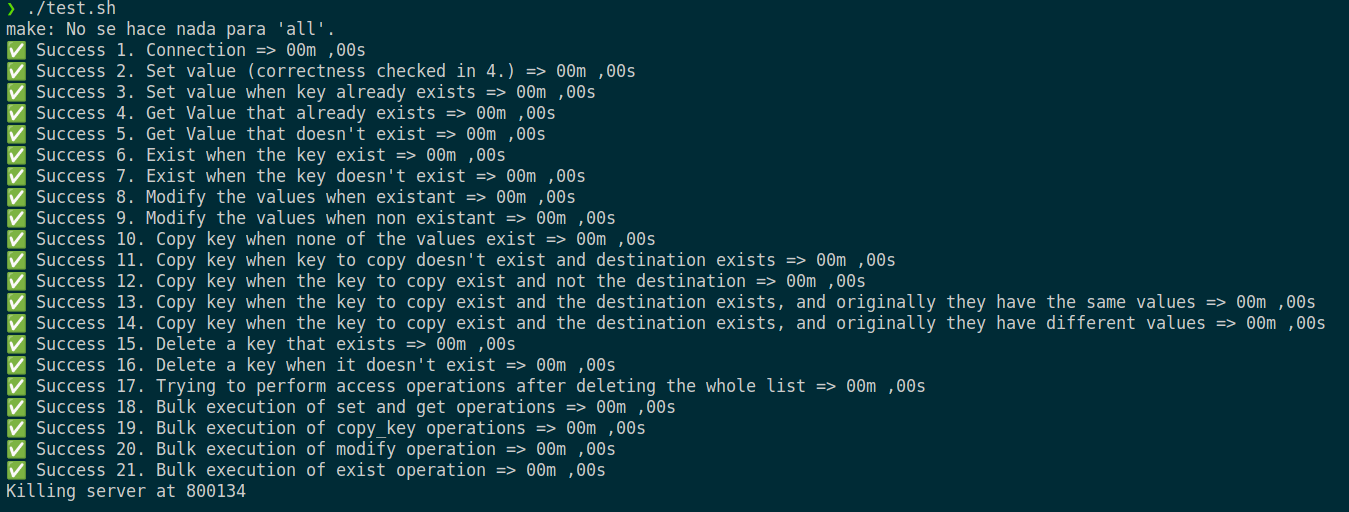
\includegraphics[width=\textwidth]{img/tests.png}
    \caption{Resultado tras ejecutar el banco de pruebas implementado para esta práctica.}
    \label{fig:tests}
\end{figure}

Como se puede ver en la figura, se han desarrollado un total de 21 pruebas destinadas a comprobar distintos casos de uso. Las primeras 17 están diseñadas para comprobar la funcionalidad de la interfaz requerida por el enunciado, tanto en caso de éxito como en caso de que la funcionalidad se esté usando indebidamente. 

Especificamente, comprobamos el borrado de las estructuras usando init, añadir tuplas, recuperar tuplas, la existencia de las tuplas, modificar tuplas y  todos los distintos casos de copiar los valores de una key en otra (existente o no).
El último test de esta categoría comprueba que se haya realizado correctamente el borrado del estado tras una llamada a \textit{init()}.

Los últimos cuatro tests tienen de nombre "bulk execution" debido a que se lanzan las operaciones pero en gran volumen (por cada operación, esta se lanza un total de 1000 veces). Adicionalmente, también se tiene la lógica de comprobar los valores por cada tupla del test (lo cual añade todavía más volumen de operaciones). Estos tests están especialmente diseñados para encontrar problemas con la conexión de sockets.

Adicionalmente, para lanzar los tests se han implementado dos ficheros llamados \textit{test.sh} y \textit{test\_async.sh} que se encargan de lanzar el servidor, lanzar el ejecutable descrito anteriormente que ejecuta las pruebas y finalmente matar el servidor (todo ello de manera automática, añadiendo las variables de entorno necesarias para su comunicación).
El primero de ellos solo lanza un banco de pruebas, mientras que el segundo lanza varios que se ejecutan paralelamente al mismo tiempo, y están destinados a comprobar problemas de concurrencia en el servidor.
Ambos bancos de pruebas (serial y concurrente) pasan sin errores.

